\subsection{One Tau lepton final state}
\label{sec:oneT}

Events fall into the one $\tau$ category if they contain at least one diphoton candidate, 
exactly one hadronically decaying tau lepton, and exactly zero electrons and muons. 

In order to maximize the sensitivity of this final state, a similar method to that of the semi-leptonic final state described in Section \ref{sec:oneL} is followed. Namely, two multiclass deep neural networks (DNNs) are trained. In this case, the structure of the DNNs are the same as those from the semi-leptonic analysis, with the electron and muon input features replaced by the $\tau$ candidate's input features. The multiclass DNNs output three scores, but only the one which estimates the likelihood that an event is HH like is used in this analysis. The distribution of this DNN score is shown in Figure \ref{fig:tau_perf}.

\begin{figure}[!htb]
    \centering
    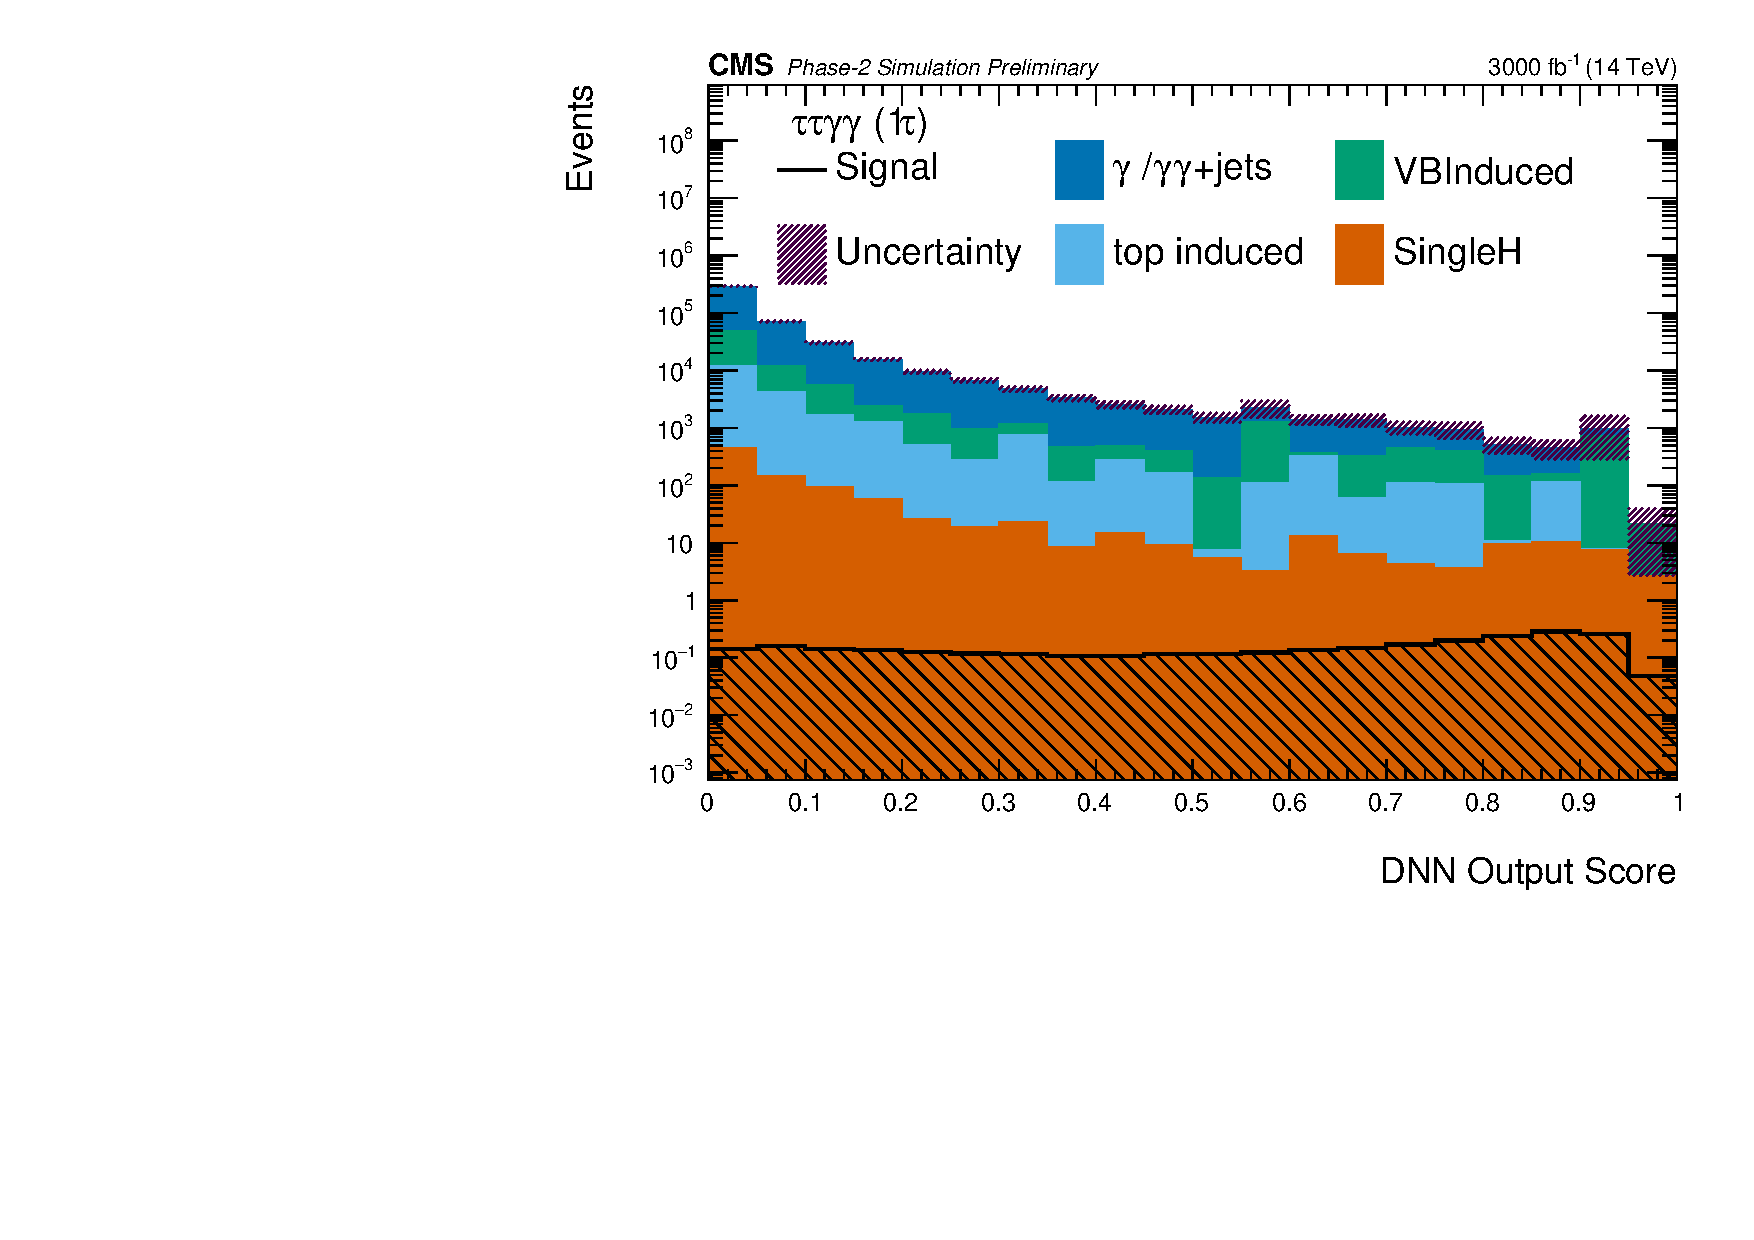
\includegraphics[width=0.75\textwidth]{Sections/Phase_II_HH/images/DNN/DNN_Score_tt_logy.pdf}
    \caption{One tau DNN output score distribution.}
    \label{fig:tau_perf}
\end{figure}

Events are partitioned into two categories based on the DNN score. Category one corresponds to events where the DNN score lies between 0.1 and 0.65, while events with a DNN score higher than 0.65 are placed into category 2. 


